\subsection{Adimensionnement de l'équation de Poisson}
%	Pour adimensionner l'énergie, nous allons nous servir de la quantité $\sigma^2$. % qui à la dimension d'une énergie.
%	Nous introduisons la quantité $r_c$, pour adimensionner les distances, puis
%	nous faisons donc le changement de variable suivant:
	L'adimensionnement des énergies se fait au moyen de $\sigma^2$ et celui des longueurs via $r_c$, en posant:
	\begin{align*}
			\gamma = \dfrac{\phi}{\sigma^2}
			\quad \mathrm{et}\quad 
			x = \dfrac{r}{r_c}
	\end{align*}

	Il vient alors:
	\begin{equation}
		\frac{d}{dx}\(x^2\frac{d\gamma}{dx}\) = -\frac{4m\pi G r_c^2 \rho_0}{\sigma^2}x^2 \left\{-\sqrt{\frac{4\gamma}{\pi}}\(1 + \frac{ 2\gamma }{3}\) + e^{\gamma}\mathrm{erf}\(\sqrt{\gamma}\)\right\}
	\end{equation}

	L'adimensionnement est complet en prenant comme chaque fois dans ce contexte:
	\begin{equation}
		r_c^2 = \frac{\sigma^2}{4m\pi G\rho_0}
		\label{r_c}
	\end{equation}
	L'équation de Poisson a résoudre numériquement s'écrit finalement:
	\begin{equation}
		\frac{d}{dx}\(x^2\frac{d\gamma}{dx}\) = x^2\frac{d^2\gamma}{dx^2} +
		2x\frac{d\gamma}{dx} = -x^2 \left\{-\sqrt{\frac{4\gamma}{\pi}}\(1 + \frac{ 2\gamma }{3}\) + e^{\gamma}\mathrm{erf}\(\sqrt{\gamma}\)\right\}
		\label{Pois-no_dim}
	\end{equation}

\subsection{Conditions aux limites et paramètres du modèle}
	
			Le système étant isolé et à l'équilibre, son centre d'inertie est au repos. Sa symétrie
			sphérique implique que la résultante des forces qui s'applique à une particule test située en
			$r=0$ s'annule. Cette force est proportionnelle au gradient du potentiel, nous avons donc:
			\begin{equation}
				\left.\frac{d\gamma}{dr}\right|_{r=0} = \left.\frac{d}{dr}\(\frac{E_l - m\psi}{\sigma^2}\)\right|_{r=0} = -\frac{m}{\sigma^2}\left.\frac{d\psi}{dr}\right|_{r=0} = 0
			\end{equation}
			En l'absence de vitesse, l'énergie minimale est atteinte pour la plus petite valeur de $m\psi(r)$, soit $m\psi(0)$.

			La quantité $\phi(r)=E_l-m\psi(r)$ représente la quantité d'énergie qu'il faut fournir à une particule située à la distance $r$
			du centre du système afin qu'elle sorte du système. 
			Il est clair que le potentiel $\psi(r)$ est une fonction partout négative ou nulle, ainsi
			$\phi(r)$ est à l'inverse positive ou nulle. Au centre, cette quantité vaudra:
			\begin{align*}
				\phi(0)=E_l-m\psi(0)
			\end{align*}

			Il est donc commode d'introduire la quantité adimensionnée:
			\begin{equation}
				W_0 = \gamma(0)=\frac{E_l - m\psi(0)}{\sigma^2} > 0
				\label{W_0}
			\end{equation}

			Nous éviterons de la prendre nulle, car, dans ce cas, le système ne contient au
			plus aucune étoile!

	Le choix de $\gamma(0)=W_0$ et le fait que la dérivée de $\gamma$ en $r=0$ soit nulle permettent la résolution numérique de
	l'équation~\refeq{Pois-no_dim}. Cette résolution permet d'obtenir le rayon $R$ de la sphère de King, premier zéro de la fonction $\phi(r)$. La
	vitesse d'une particule test située en $r=R$ est la vitesse de libération du système, en introduisant $X=\frac{R}{r_c}$ nous avons bien:
		\begin{equation}
			 E_l = m\psi(X) \;\Leftrightarrow\; \gamma(X) = 0
		\end{equation}

	Le paramètre $W_0$ fixe donc toutes les caractéristiques nécessaires à la résolution numérique du modèle de King. Le rayon de la sphère de
	King est une fonction croissante de $W_0$. Comme nous pouvons le voir sur la définition~\refeq{W_0}, une même valeur de $W_0$ peut correspondre à
	des systèmes possédant des caractéristiques physiques différentes caractérisées par une profondeur du puits de potentiel $\psi(0)$, une
	dispersion de vitesse $\sigma^2$ ou une énergie de libération différente. Ces différences ne concernent que le système une fois redimensionné. 

\subsection{Résolution numérique}
	L'algorithme que nous utiliserons pour résoudre l'équation~\refeq{King-Pois} est un Runge-Kutta
	d'ordre $4$ (RK4). Nous devons écrire l'équation différentielle comme un système d'ordre 1, ce que nous faisons en posant $u = \frac{d\gamma}{dx}$:
	\begin{equation}
		\left\{\begin{array}{l}
			u = \x{\gamma}\\
			\\
			\x{u} = -\left\{-\sqrt{\frac{4\gamma}{\pi}}\(1 + \frac{ 2\gamma }{3}\) + e^{\gamma}\mathrm{erf}\(\sqrt{\gamma}\)\right\} - 2\frac{u}{x}
		\end{array}\right.\label{sys2dking}
	\end{equation}

%	Euh .... Outre un problème évident de division par zéro en $x=0$, qui peut-être résolu à
%	l'aide d'un développement limité du potentiel au centre, lors de l'intégration, la solution
%	pour le potentiel est positive !!! \textcolor{red}{$\Rightarrow$ Normal, j'ai
%	oublié de repasser au potentiel !!! Je trace $\gamma$, et non $\psi$, qui est forcément
%	positif !!!}
	Un terme en $1/x$ est apparu, l'équation semble donc singulière en $0$. Un 
	développement limité de la fonction $\gamma$ autour de $0$ nous apprend qu'il n'en est rien, il n'y a
	pas de divergence. Un rapide calcul montre que toutes les dérivées d'ordre impair de $\gamma(x)$ s'annulent en $x=0$, et que:
	$$
	\gamma(0) = W_0\, ,\;\; \gamma''(0) = -\frac{\rho(W_0)}{3\rho_0}\; \mathrm{et}\; \gamma^{(4)}(0) = \frac{2\rho(W_0)}{5\rho_0}\left\{\sqrt{\frac{W_0}{\pi}} -
			\frac{e^{W_0}\mathrm{erf}(\sqrt{W_0})}{2}\right\} 
	$$
	Nous pouvons donc écrire directement un développement de Taylor de $\gamma(x)$ à l'ordre 5 en $x=0$. 
	La résolution des équations nous permet alors d'avoir les graphiques de la
	figure~\ref{King_Modele-test} (les graphiques sont adimensionnés).% mais pas normalisé~).
%	\paragraph{Problème: Résolu:}
%	Tant que la variable $x$ est proche de $0$, j'utilise les développements limités, puis passé
%	un certain seuil, je réutilise l'équation différentielle. Le résultat obtenu est la figure~\ref{King_Modele-err}
%	au lieu de la figure~\ref{King_Modele} (~figure pour laquelle je démarre à $x=1.10^{-6}$ au
%	lieu de $x=0$~). Il semblerait que mon algorithme de RK4 à pas variable ait du mal à suivre,
%	en plus d'avoir, apparemment, une erreur d'adimensionnement/normalisation.
%	\subparagraph{Solution pour le RK4 ne suivant pas:} J'utilisais le développement de $\gamma(x)$ pour calculer la pente
%	et celui de $\x{\gamma(x)}$ pour calculer la dérivée seconde.

%	\textcolor{red}{RAAAAAAHHHHHHHHH !!!!!!!!!! Plein d'erreur de signe dans les calculs et le
%	programme !!!!!!!!!!! Faut tout revérifier !!!!!!!!!!!!!!!!!!!}

%	\begin{figure}[ht!]
%			\begin{minipage}[b]{0.40\linewidth}
%				\centering 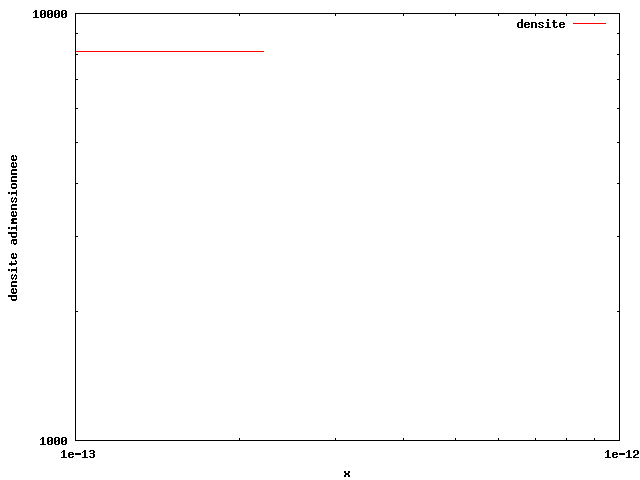
\includegraphics[scale=0.40]{graphe/erreur_king.png}
%			\end{minipage}\hfill
%			\begin{minipage}[b]{0.48\linewidth}
%				\centering 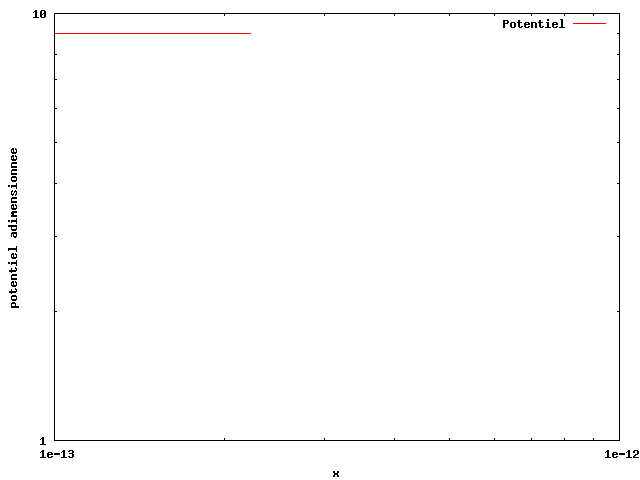
\includegraphics[scale=0.40]{graphe/erreur-pot_king.png}
%			\end{minipage}
%			\caption{Densité et potentiel d'un modèle de \textsc{King} pour les
%			conditions initiales (~au centre~): $\gamma(0) = \frac{E_l -
%			m\psi(0)}{\sigma^2} = 9$}
%			\label{King_Modele-err}
%	\end{figure}
%	\begin{figure}[ht!]
%			\begin{minipage}[b]{0.40\linewidth}
%				\centering \includegraphics[scale=0.60]{graphe/densite_king.pdf}
%			\end{minipage}\hfill
%			\begin{minipage}[b]{0.48\linewidth}
%				\centering \includegraphics[scale=0.60]{graphe/potentiel_king.pdf}
%			\end{minipage}
%			\caption{Densité et potentiel d'un modèle de \textsc{King} pour les
%			conditions initiales (~au centre~): $\gamma(0) = \frac{E_l - m\psi(0)}{\sigma^2} = 3$, $\x{\gamma}(0) = 0$}
%			\label{King_Modele}
%	\end{figure}

	\begin{figure}[ht!]
			\begin{minipage}[b]{0.40\linewidth}
				% \centering \includegraphics[scale=0.60]{graphe/densite_pluri-king.pdf}
				\centering 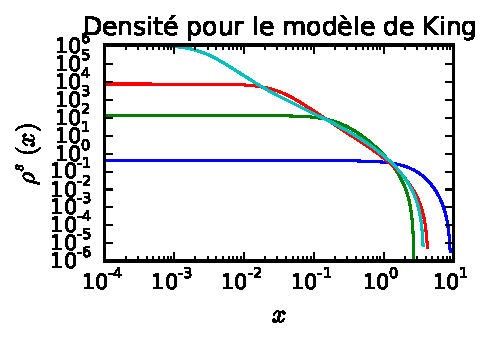
\includegraphics{graphe/king.pdf}
			\end{minipage}\hfill
			\begin{minipage}[b]{0.48\linewidth}
				% \centering \includegraphics[scale=0.60]{graphe/densite_pluri_limite-king.pdf}
				\centering 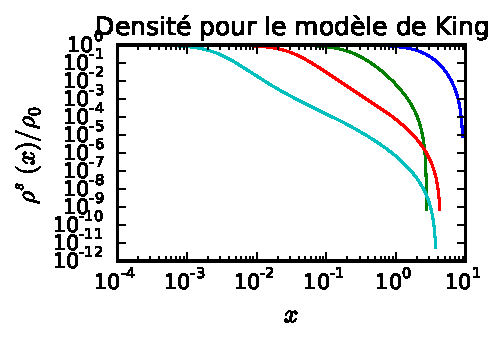
\includegraphics{graphe/king_n.pdf}
			\end{minipage}
			\caption{Différents profil de densité pour un modèle de King. En bleu foncé: $W_0=1$, en vert
			$W_0=5$, en rouge $W_0=9$ et en bleu clair $W_0=14$.\label{King_Modele-test}}
	\end{figure}

	%La figure~\ref{King_Modele-test} montre l'aspect de la densité d'un modèle de \textsc{King} en fonction de $W_0$ et nous indique aussi que ce modèle posséde une structure cœur-halo
	%(~une partie quasiment constante suivi d'une décroissance auto-similaire de pente $\alpha$~).
	%Plus $\phi$ est grand, plus le cœur est dense (~le graphe de droite trace $\rho(x)/\rho(0)$~). Nous pouvons aussi observer que la pente n'est pas la même:
	%elle diminue (~la courbe tend plus vite vers $0$~). Ce constat nous amène à nous poser une question: existe-t-il un
	%lien entre la pente et le rayon du cœur ?
	
	La résolution numérique du système~\refeq{sys2dking} permet d'obtenir la fonction $\gamma(x)$ pour chaque donnée
	initiale $W_0$. De cette fonction nous en déduisons la densité volumique de masse du système adimensionnée $\rho^s(x)$ par la relation:
	\begin{align*}
		\rho^s(x) = \dfrac{\rho(x)}{\rho_0} = e^{\gamma(x)} \mathrm{erf}\(\sqrt{\gamma(x)}\) - \sqrt{\dfrac{4\gamma(x)}{\pi}}\(1+\dfrac{2\gamma(x)}{3}\)
	\end{align*}
	% Une sphère de King adimensionnée est donc entièrement définie par le paramètre $W_0$.
	En échelle
	logarithmique, sa densité normalisée est très bien approchée sur plus de 5 décades par deux segments de droites
	: l'un horizontal décrit le cœur de la sphère de densité quasiment constante, l'autre de pente $-\alpha$
	décrit un halo autosimilaire entourant le c\oe ur. L'intersection des droites portant ces deux segments est une
	bonne approximation de ce que l'on pourrait appeler le rayon du c\oe ur de la sphère de King considérée.

	Pour les petites valeurs de $W_0$, typiquement $W_0\leq 5$, la sphère
	de King est essentiellement constituée d'un très large c\oe ur de
	densité quasiment constante. Par contre dès que  $W_0\geq 15$, le c\oe
	ur ne renferme plus qu'une faible proportion de la masse du système et
	la sphère de King est essentiellement constituée d'un halo
	autosimilaire dont la densité est comparable à celle d'une sphère
	isotherme singulière. Cette comparaison n'est valide que jusqu’à un certain rayon
	où la densité de la sphère de King chute violemment  à cause de la
	troncature introduite par l'énergie de libération. Une étude plus fine
	montre que les halos des sphères de
	King sont associés à des profils autosimilaires de pente étagée entre
	$-5$  et $-2$ lorsque $W_0$ varie de $5$ à $15$. La figure~\ref{coeff_evo} illustre ce comportement.
	
	\begin{figure}[hbt!]
%		\centering \includegraphics[scale=1.00]{../Resol_King/img-king/pente-w0.pdf} %{graphe/evo-coeff_ci.pdf}
		% \centering \includegraphics[scale=1.00]{graphe/pente-w0.pdf}%{img-king/pente-w0.pdf} %{graphe/evo-coeff_ci.pdf}
		\centering 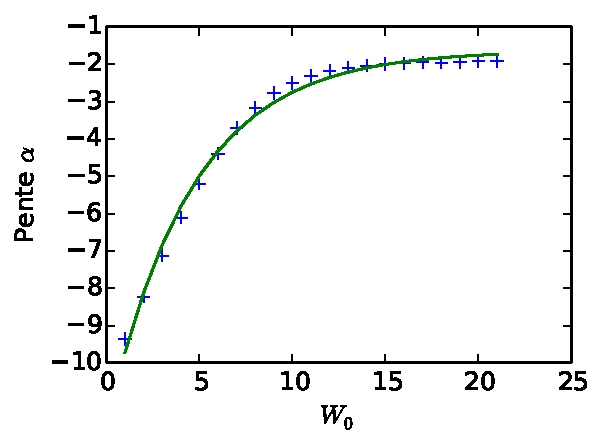
\includegraphics{king_pente_w0.pdf} %{graphe/pente-w0.pdf}%{img-king/pente-w0.pdf} %{graphe/evo-coeff_ci.pdf}
		\caption{Évolution de la pente du halo de la sphère de King en fonction de $W_0$}
		\label{coeff_evo}
	\end{figure}
	
	Une sphère de King définie par une grande valeur de $W_0$ est donc très
	proche d'une sphère isotherme singulière, sa température est donc
	vraisemblablement indépendante de la distance au centre. Il est
	intéressant de préciser cette idée de façon plus quantitative. C'est
	l'objet de la prochaine section.
	
	% \FloatBarrier
